%\newpage
% -----------------------------------------------------------------------
\chapter{Coursework}
%-----------------------------------------------------------------------
\section{Introduction}
A project will cover most of the topics from this course. At the end
of each chapter, there will be a set of exercises which are used to
strengthen the knowledge in software engineering. In addition, each
student will have the possibility to play around with the tools
demonstrated in this course.\\
For all the coursework, each student needs to have a computer
(Windows, OSX or Linux) with the possibility to install additional
software.

\subsection{Projects}
There are two projects available. The two projects are
developed for the following two courses:

\begin{itemize}
\item Gene Information Service (FHNW - Master Medical Informatics)
\item Raspberry Pi GPIO Web Application (FHNW - Master Automation Management)
\end{itemize}


\section{Gene Information Service}
The gene information service will be a system with three components:

\begin{itemize}
\item Data Loader\\
This component loads a data file from NCBI into a database
\item Gene Information Service\\
This component will provide a REST based service which could
be used by other applications to retrieve gene specific information
\item Gene Search Web Application
This component will provide a simple Java based Web Application
which utilizes the Gene Information Service
\end{itemize}

\section{What is a gene}
In biology, a gene is a sequence of nucleotides in DNA or RNA that encodes the
synthesis of a gene product, either RNA or protein.\\
(Source: Gene: Wikipedia)

\begin{centering}
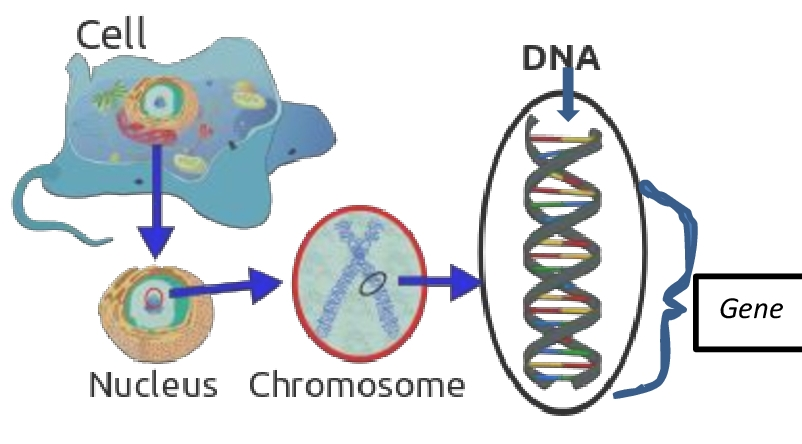
\includegraphics[width=250pt]{images/coursework/geneinfo.jpg}\\
\end{centering}

\section{Basic Idea}
The gene information service will provide a system to retrieve
information for a given gene.
\begin{itemize}
\item The data which is used is coming from NCBI. The raw data size
is in the area of 4GB.
\item This data will be loaded into a database (e.g. MySQL, Postgres).
This will be done by the first component, \emph{Data Loader}
\item The data will be available over a REST interface. This is
the second component. The service will be connected to the database
a will provide query functionalities for end users.
\item A end user application will be created, where potential
users could create queries and display the gene information data.
This could be a web application or also a mobile application. In this
project, we will use a web application.
\end{itemize}

\section{Exercises}
\begin{enumerate}
\item In each project it is important to understand the data which
is used. Download the gene information file from the NCBI ftp server:\\
\vspace{3mm}
\verb|ftp://ftp.ncbi.nlm.nih.gov/gene/DATA/gene_info.gz|\\
\vspace{3mm}
Try to answer the following questions:
\begin{itemize}
\item How many genes does the file contain?
\item What kind of information is in the \verb|tax_id| field?
\item Which gene types do exist?
\item Which gene type is the one which appears the most?
\end{itemize}

\end{enumerate}
